% =========================================================================
% Hand-Drawn Circuit Diagram to SPICE: A Verified Benchmark on Digitize-HCD
% with Structural Connectivity Recovery and Transparent Design-Intent Repair
%
% IEEE Access submission draft. SCAFFOLD + DRAFT for Ammaar Junaid's
% revision — the scholarly voice is the author's; nothing here is final.
%
% Build: drop this directory into the official IEEE Access Overleaf
% template (ieeeaccess.cls). Falls back to IEEEtran [journal] so the
% draft also compiles in a plain TeX Live.
%
% HARD RULE (project convention): no hand-typed numbers anywhere in the
% prose or tables. All numbers come from paper/generated/*.tex, produced
% by scripts/make_paper_tables.py from committed results/ artifacts.
% Regenerate with:  python scripts/make_paper_tables.py
% =========================================================================
\IfFileExists{ieeeaccess.cls}{%
  \documentclass{ieeeaccess}%
}{%
  \documentclass[journal]{IEEEtran}%
}
\usepackage{cite}
\usepackage{amsmath,amssymb,amsfonts}
\usepackage{graphicx}
\usepackage{booktabs}
\usepackage{tikz}
\usetikzlibrary{positioning,arrows.meta,shapes.geometric,fit,backgrounds}
\usepackage{xcolor}
\usepackage[colorlinks=true,linkcolor=blue,citecolor=blue,urlcolor=blue]{hyperref}

% ---- numbers generated from results/ (never hand-typed) -----------------
% AUTO-GENERATED by scripts/make_paper_tables.py — do not edit.
% Regenerate after any results change.
\newcommand{\NumTestImages}{190}
\newcommand{\SupportMin}{44}
\newcommand{\SupportMinClass}{MOSFET-P}
\newcommand{\SupportMax}{448}
\newcommand{\SupportMaxClass}{Resistor}
\newcommand{\NumClasses}{17}
\newcommand{\OracleDetection}{+0.0339}
\newcommand{\OracleWires}{+0.4368}
\newcommand{\OracleSnapping}{+0.0084}
\newcommand{\OracleNValid}{160}
\newcommand{\RepLiftCiLo}{0.295}
\newcommand{\RepLiftCiHi}{0.432}
\newcommand{\RepRegressed}{0}
\newcommand{\RepTopoViolations}{0}
\newcommand{\RepVerifiedImages}{190}
\newcommand{\GroundAccResolved}{0.821}
\newcommand{\GroundAccStrict}{0.650}
\newcommand{\GroundNGnd}{183}
\newcommand{\DetMapFifty}{0.972}
\newcommand{\DetMapFiftyStd}{0.0012}
\newcommand{\DetMapFiftyNinetyFive}{0.727}
\newcommand{\AblNetFOneClassical}{0.433}
\newcommand{\AblNetFOneVFive}{0.637}
\newcommand{\AblTpFOneClassical}{0.163}
\newcommand{\AblTpFOneVFive}{0.463}
\newcommand{\RepSolvBefore}{0.353}
\newcommand{\RepSolvAfter}{0.716}
\newcommand{\RepMeanAssumptions}{4.0}
\newcommand{\RepMeanGauge}{1.7}
\newcommand{\RepSpiceValid}{0.979}


% ---- draft-status helpers (strip before submission) ---------------------
\newcommand{\todoa}[1]{\textcolor{red}{[TODO Ammaar: #1]}}
\newcommand{\draftnote}[1]{\textcolor{orange}{[draft note: #1]}}

\begin{document}

\title{A Verified Benchmark for Hand-Drawn Circuit Diagram to SPICE
Netlist Conversion on Digitize-HCD, with Structural Connectivity
Recovery and Transparent Design-Intent Repair}

% IEEE Access uses \author{\uppercase{...}} with \authorrefmark and a
% \corresp block — restore those when moving into the official template.
\author{Ammaar~Junaid% \authorrefmark{1}
\thanks{\todoa{affiliation, ORCID, corresponding-author email, and the
authorship decision (mentor per IEEE's three criteria).}}%
}

% \history{...} % IEEE Access template command — dates filled by portal.
% \doi{...}

\markboth{IEEE Access, draft of \today}{Junaid: Verified Benchmark for
Hand-Drawn Circuit to SPICE on Digitize-HCD}

\maketitle

\begin{abstract}
Converting a photographed, hand-drawn circuit diagram into a machine-
readable SPICE netlist requires recovering symbols, wiring topology, and
electrical intent from noisy freehand strokes. Despite a growing
literature, no public evaluation benchmark with human-verified
connectivity ground truth exists for this task: prior systems report
results on private or unreleased test sets, making claims incomparable.
We present the first published benchmark on the public Digitize-HCD
dataset: frozen splits, human-verified ground-truth topology for all
\NumTestImages{} test images, a standardized metric cascade (detection
mAP, terminal-pair $F_1$, net-level $F_1$, normalized graph edit
distance, strict end-to-end success, SPICE validity and DC solvability),
and released code that regenerates every reported number. On this
benchmark we develop a lightweight local pipeline whose connectivity
stage is progressively strengthened — binarized-ink wire extraction,
mask-hole stitching, crossover-aware net assembly driven by the
detector's \emph{Wire Crossover} class, and constraint-triggered
connectivity repair — improving net-level $F_1$ from
\AblNetFOneClassical{} (classical baseline) to \AblNetFOneFinal{} and
strict end-to-end success from \AblStrictClassical{} to
\AblStrictFinal{}, with each step validated by paired per-image
bootstrap tests. A
GT-injection oracle attributes the remaining error to individual
stages. Finally, we introduce a transparent design-intent repair layer:
electrical rule checks diagnose why a recovered circuit cannot be
simulated, and a minimal, fully-logged set of repairs — each classified
as a behavior-invariant \emph{gauge} choice or a flagged
\emph{assumption} with alternatives — raises DC solvability from
\RepSolvBefore{} to \RepSolvAfter{} while provably leaving the
recovered topology untouched. \draftnote{abstract $\le$250 words;
recheck after final numbers land.}
\end{abstract}

\begin{IEEEkeywords}
\todoa{pick 3--10 from the IEEE Thesaurus} circuit topology extraction,
document image analysis, hand-drawn schematics, netlist generation,
object detection, SPICE simulation
\end{IEEEkeywords}

\IEEEpeerreviewmaketitle

\section{Introduction}
\label{sec:introduction}

% Draft for Ammaar's revision. Voice: measured, claims scoped to what
% the artifacts support. Every number is a generated macro.

\IEEEPARstart{H}{and-drawn} circuit diagrams remain the lingua franca
of electronics education, whiteboard design discussions, and lab
notebooks. Converting a photograph of such a sketch into a
machine-readable SPICE netlist would connect this informal medium
directly to simulation, checking, and documentation tools. The task is
deceptively hard: it requires detecting freehand component symbols,
tracing noisy, gapped, and crossing pencil strokes into electrical
nets, associating component terminals with those nets, and finally
emitting a netlist that a simulator will actually accept.

Recent systems report strong headline results on this task
\cite{wang2026topology,sina2026,reddy2022handdrawn}, yet the field has
a reproducibility problem: to our knowledge, \emph{no public
evaluation benchmark with human-verified connectivity ground truth
exists}. Wang et al.\ \cite{wang2026topology} train on the public
Digitize-HCD dataset \cite{digitizehcd_data} but evaluate on an
independent 1{,}317-image benchmark that is not released; SINA
\cite{sina2026} and Netlistify \cite{netlistify} evaluate on their own
curated sets. Published numbers are therefore not comparable, and none
of the underlying ground truth is available for scrutiny. Separately,
most pipelines stop at topology: whether the emitted netlist actually
\emph{simulates} — and what silent assumptions were needed to make it
simulate — is rarely measured or disclosed.

This paper addresses both gaps. Our contributions are:

\begin{enumerate}
  \item \textbf{C1 — the first published evaluation benchmark on
  Digitize-HCD.} Frozen train/val/test splits (895/192/\NumTestImages),
  human-verified ground-truth topology for every test image, a strict
  GT validator, and released code that regenerates every number in
  this paper. Digitize-HCD has been used for \emph{training}
  \cite{wang2026topology}; nobody has published an evaluation protocol
  or baseline results on it.

  \item \textbf{C2 — structural connectivity recovery that measurably
  beats classical CV.} A progression of interpretable connectivity
  stages — binarized-ink wire extraction, stitching of mask-induced
  wire gaps, and crossover-aware net assembly driven by the detector's
  \emph{Wire Crossover} class — lifts net-level $F_1$ from
  \AblNetFOneClassical{} to \AblNetFOneVFive{} and terminal-pair $F_1$
  from \AblTpFOneClassical{} to \AblTpFOneVFive{}, with every step
  validated by a paired per-image bootstrap test.

  \item \textbf{C3 — port-aware terminal handling.} Class-aware
  terminal semantics (pin identity and polarity for directional
  two-terminal parts) derived from Digitize-HCD's port-location
  annotations, an annotation modality no published work exploits.
  \draftnote{scope this bullet to exactly what lands in
  Sec.~\ref{sec:method}; MSP = two-terminal polarity + pin order.}

  \item \textbf{C4 — metric standardization and stage attribution.} A
  metric cascade from detection mAP through terminal-pair/net $F_1$,
  normalized graph edit distance, strict end-to-end success, SPICE
  validity, and DC solvability, reported together with bootstrap
  confidence intervals; plus a ground-truth-injection oracle that
  attributes end-to-end error to individual pipeline stages.

  \item \textbf{C5 — transparent, minimal design-intent repair.} An
  electrical-rule-check layer diagnoses why a recovered circuit cannot
  be DC-solved, and a repair layer applies the \emph{minimal} set of
  explicit fixes, each logged in a human-reviewable assumption ledger
  and classified as a behavior-invariant \emph{gauge} choice or a
  flagged, behavior-changing \emph{assumption} with alternatives.
  Repair raises DC solvability from \RepSolvBefore{} to
  \RepSolvAfter{} while provably never altering the recovered
  topology.
\end{enumerate}

Together these turn an anecdotally-evaluated task into a measured one:
the benchmark quantifies exactly where current pipelines fail (wire
topology and terminal association, not symbol detection — detection is
essentially solved at \DetMapFifty{} mAP@0.5), and the repair layer
makes the final, usually-hidden step from ``topologically plausible''
to ``simulable'' explicit and auditable.

\draftnote{closing paragraph: one-sentence paper roadmap.}

\section{Related Work}
\label{sec:related}

% Draft for Ammaar's revision. Positioning rules (from the plan):
% - C5 must be positioned against ERC/convergence-aid prior art
%   honestly, NOT overclaimed as "unlike any software".
% - Claim "first PUBLISHED benchmark on Digitize-HCD", not "first to use".

\subsection{Hand-Drawn Circuit Recognition Pipelines}
Early work treated the task as symbol recognition plus ad-hoc wire
tracing. Reddy and Panicker \cite{reddy2022handdrawn} combine YOLOv5
component detection with Hough-based node recognition and report
98.2\% detection mAP@0.5, but evaluate connectivity only qualitatively
on a small private set. Recent end-to-end systems are stronger: SINA
\cite{sina2026} couples detection, connected-component connectivity
reasoning, OCR, and a vision-language model for designator assignment;
Netlistify \cite{netlistify} adds orientation detection to component
recognition. Wang et al.\ \cite{wang2026topology} is closest to our
setting: a topology-consistent parsing framework trained on
Digitize-HCD with wire connected-component-guided connectivity and
explicit endpoint semantics, reporting a 95.14\% strict image-level
success rate. In all of these, however, evaluation is performed on
private or unreleased test sets with bespoke metrics, so results
cannot be compared or audited. Our contribution is deliberately
complementary: a frozen, human-verified, public evaluation protocol
(C1/C4) plus baseline results, against which such systems can be
measured.

\subsection{Datasets and Graph Extraction on CGHD}
Two public datasets anchor the field. CGHD \cite{cghd} provides
hand-drawn circuit images by multiple drafters with symbol bounding
boxes, and later releases add segmentation maps; the accompanying line
of work by Bayer et al.\ extracts electrical graphs via instance
segmentation \cite{bayer2023instance}, modular pipelines
\cite{bayer2024modular}, and text extraction \cite{bayer2023text}.
Digitize-HCD \cite{digitizehcd_data} contributes 1{,}277 photographed
hand-drawn circuits with 18{,}600 component boxes over 17 classes,
text transcriptions, and — uniquely — per-class \emph{port-location}
annotations (Gaussian heatmaps and pixel coordinates). Neither dataset
ships connectivity ground truth for end-to-end evaluation; our
benchmark adds exactly that layer on Digitize-HCD, and we use CGHD's
class dictionary for a cross-dataset mapping. \draftnote{mention the
P\&ID/engineering-drawing digitization literature in one sentence if a
survey ref is added to refs.bib.}

\subsection{Making Recovered Circuits Simulate}
That a syntactically valid netlist can still fail DC analysis is a
classic problem: simulators ship convergence aids (gmin stepping,
source stepping, \texttt{.nodeset}) \cite{ngspice}, and schematic
tools ship electrical rule checks (ERC) that flag floating nodes or
missing references. Our C5 layer builds deliberately on this prior
art rather than claiming novelty over it: what is new is (i) applying
ERC-style diagnosis to \emph{recovered} (noisy, machine-inferred)
circuits rather than human-entered ones, (ii) enforcing a
\emph{minimality} discipline over the applied fixes, and (iii) the
\emph{assumption ledger} — a per-circuit, machine-readable record that
classifies each repair as behavior-invariant (\emph{gauge}) or
behavior-changing (\emph{assumption}), with alternatives, so a human
can audit exactly what the system assumed about their design intent.
To our knowledge no published hand-drawn-circuit system measures or
discloses this repair step; they either report simulation success
without stating what was fixed, or stop at topology.

\section{Dataset and Ground Truth}
\label{sec:dataset}

% Draft for Ammaar's revision. Facts sourced from data/README.md,
% docs/GT_VERIFICATION_GUIDE.md, and the split manifests — keep in sync.

\subsection{Source Dataset}
Digitize-HCD \cite{digitizehcd_data} (CC BY 4.0) contains 1{,}277
photographs of hand-drawn circuit diagrams at roughly 2000\,px
resolution, annotated with 18{,}600 COCO-format component bounding
boxes over 17 classes (BJT-NPN/PNP, capacitor, diode, Zener diode,
GND, AC/DC current and voltage sources, one-port DC source, inductor,
MOSFET-N/P, op-amp, resistor, and \emph{Wire Crossover}), MMOCR-style
text annotations with transcriptions, and per-class component crops
with port-location Gaussian heatmaps and pixel port coordinates. We
verified our copy byte-for-byte against the published archive (SHA-256
of the 2.1\,GB release; every one of the 1{,}277 images matched).

The COCO records carry no drafter identity, so drafter-disjoint
splitting is impossible — a stated limitation of any benchmark on this
dataset. We instead freeze a stratified split of 895/192/\NumTestImages{}
(train/val/test), stratified by component-count tertile and
rarest-class presence; all \NumClasses{} classes appear in every split,
with test-set support ranging from \SupportMin{}
(\SupportMinClass) to \SupportMax{} (\SupportMaxClass) instances
(Table~\ref{tab:detection}). The split manifests are versioned with the
code.

\subsection{Preprocessing and Coordinate Frames}
All stages operate on a \emph{cleaned frame}: deskew (length-weighted
median of Hough segment angles folded mod $90^\circ$, with a robust
fallback), shadow normalization, binarization, a content crop, and an
aspect-preserving resize onto a $512\times512$ canvas. Two properties
make this frame benchmark-safe. First, the full geometric transform of
every image is recorded, so published original-frame annotations
project exactly into the cleaned frame (verified: 0 of 18{,}600
projected boxes fall off-canvas, enforced by a guard script). Second,
the crop is \emph{annotation-aware}: every annotated component is
unioned into the crop rectangle before speck removal, making it
structurally impossible for a labeled component to be cropped out.

\subsection{Human-Verified Connectivity Ground Truth}
\label{sec:gt}
Digitize-HCD ships no connectivity ground truth, so we created it for
both evaluation splits. Each GT file is a component-terminal graph: per
component, a class, a bounding box, and per-terminal net assignments
(ground is always net~0), under a strict schema with a validator that
rejects unnamed terminals, single-terminal nets, and class/terminal
arity mismatches.

Critically, the test-split annotation was \emph{not} produced by running
the pipeline and correcting its output. Component inventory and box
geometry come from the published COCO annotations; every net was traced
from \texttt{null}. Each image went through wire extraction under
hysteresis binarization, a criticality analysis that flips every
junction/crossing call and retains only the sites where the partition of
terminals changes, adjudication by eye at 5--24$\times$ magnification,
deterministic net reconstruction from the recorded decisions, an
electrical rule check, and an automated self-consistency re-derivation.
Nets are recomputed from the decision record rather than hand-edited, so
every shipped netlist is reproducible from it, and the decision records
are released alongside the netlists.

Ground truth records the topology \emph{as drawn}. Where a faithful
reading yields a circuit that cannot be simulated --- one sheet in the
test split has a rail tip landing on a grounded column, which
short-circuits a voltage source --- the annotation keeps the drawn
topology and the electrical rule check reports the fault. Electrically
motivated corrections are never folded into the topology; the
observation that a shorted voltage source appears nowhere else in the
annotated set is recorded in that file's notes as evidence about the
drawing, not as a change applied to it.

That protocol matters for more than rigor: ground truth seeded by the
pipeline's own output would make any evaluation of that pipeline
partly circular. Table~\ref{tab:gt-verification} reports the volume of
judgement it took --- every count derived from the released decision
records, not from prose --- and Table~\ref{tab:splits} gives the split
composition. Two findings from the pass are worth carrying forward: the
dominant error mode is a terminal landing on a stroke of the handwritten
value label rather than on the lead, which is why a one-terminal net is a
hard error in the rule check; and pin order on three-terminal parts was
wrong far more often than net grouping, a failure no net-level or
electrical check can detect.

The re-derivation rows of Table~\ref{tab:gt-verification} must be read
for what they are. Each sampled file was re-derived from the drawing
without reading the first pass's reasoning first, and the two netlists
were compared --- but that re-derivation was performed by an \emph{AI
assistant, not by an independent human annotator}. It is a real check on
clerical and transcription error --- formatting faults, inconsistent
terminal counts, duplicate nodes, one-terminal nets --- and it caught
them: seven of the nine files flagged by the cross-checks changed. It is
a weak check on judgement, because it shares the first pass's reasoning
and blind spots, so agreement is evidence of consistency rather than of
correctness. It is not an inter-annotator agreement study and we do not
report it as one. Independent second annotation by an external annotator
is \emph{pending}.
\todoa{external second annotation of ambiguous crossings and
three-terminal pin order — state the result here if/when it happens.}
The verified GT files and decision records are released with the
benchmark; images remain under the original Digitize-HCD license.

\begin{table}[t]
  \centering
  \caption{Split composition. Connectivity ground truth exists for both
  evaluation splits; the training split carries only the published box
  annotations.}
  \label{tab:splits}
  % AUTO-GENERATED by scripts/make_paper_tables.py — do not edit.
\begin{tabular}{lrrrrl}
\toprule
split & images & components & terminals & nets & role \\
\midrule
train & 895 & -- & -- & -- & detector training \\
val & 190 & 2576 & 5116 & 1509 & parameter selection \\
test & 192 & 2564 & 5090 & 1496 & reported, never selected on \\
\bottomrule
\end{tabular}

\end{table}

\begin{table}[t]
  \centering
  \caption{Judgement recorded while building the test-split ground truth.
  Every count is derived from the released per-image decision records by
  \texttt{scripts/gt\_verification\_stats.py}. The lower block reports an
  \emph{automated self-consistency re-derivation}: files re-derived from
  the drawing before reading the first pass, by an AI assistant and
  \emph{not} by an independent human annotator. It detects clerical and
  transcription error; it cannot establish that a judgement call is
  correct, because it shares the first pass's reasoning. Independent
  human second annotation is pending.}
  \label{tab:gt-verification}
  % AUTO-GENERATED by scripts/make_paper_tables.py — do not edit.
\begin{tabular}{lr}
\toprule
recorded decision & count \\
\midrule
intersection sites adjudicated & 2047 \\
\quad read as junction & 1707 \\
\quad read as crossing & 194 \\
\quad explicit edge grouping & 63 \\
\quad ink meets, nothing joins & 83 \\
terminals repointed to a different lead & 1261 \\
nets asserted where the box swallowed the contact & 40 \\
wire fragments re-joined across a scan gap & 38 \\
gap bridges rejected as not-touching & 3 \\
published component classes corrected & 3 \\
components marked deliberately unconnected & 1 \\
\midrule
\multicolumn{2}{l}{\emph{second reader, re-derived from the drawing first}} \\
\quad blind random & 0/12 \\
\quad stratified on sheets with 3-terminal parts (38 3-terminal parts) & 0/5 \\
\quad flagged by cross-checks & 7/9 \\
\bottomrule
\end{tabular}

\end{table}

\subsection{Cross-Dataset Material}
For context and future zero-shot evaluation we also stage CGHD
\cite{cghd} (3{,}255 images, 25 drafters) with a mapping from its
53-entry class dictionary onto the 17 Digitize-HCD categories.
\draftnote{keep only if the zero-shot experiment [IDEAL] actually runs;
otherwise fold into future work.}

\section{Method}
\label{sec:method}

% Draft for Ammaar's revision. Week-2 deliverable. Faithful to the
% implementation in src/schematic2netlist/ as of this commit; every
% threshold named here lives in configs/default.yaml (single source of
% truth) — the prose deliberately names the config keys so reviewers
% can map text to code.

Fig.~\ref{fig:pipeline} shows the pipeline: preprocessing, component
detection, wire extraction, net assembly, terminal snapping, netlist
export, and the design-intent repair layer. The design philosophy is
deliberate: a lightweight, locally-runnable system of interpretable
stages, each independently measurable (Sec.~\ref{sec:setup}) and each
switchable to its classical baseline in configuration — the ablations
in Sec.~\ref{sec:results} are config switches, not code forks.

\begin{figure*}[t]
  \centering
  % Pipeline figure (vector art, TikZ) — replaces the legacy bioRender
% flowchart. \input from main via figures/pipeline_figure.
% Two-column width (figure*). Repair layer shaded; config switches dashed.
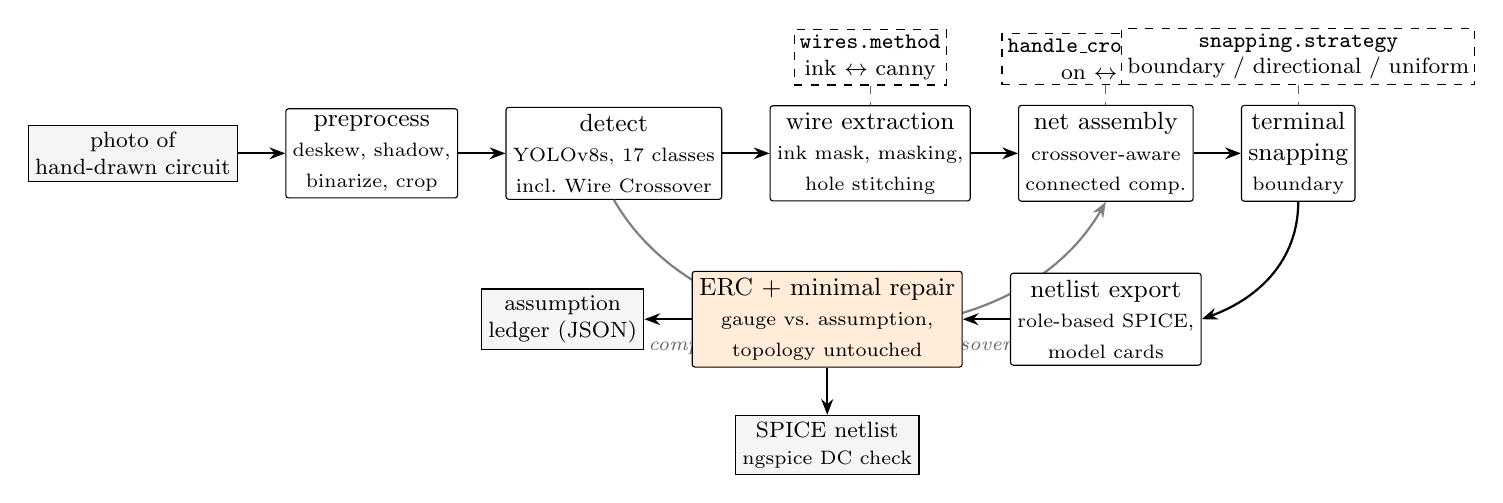
\begin{tikzpicture}[
  font=\small,
  node distance=4mm and 6mm,
  stage/.style={draw, rounded corners=1pt, align=center,
                minimum height=9mm, inner sep=2.5pt, fill=white},
  data/.style={draw, align=center, minimum height=7mm, inner sep=2.5pt,
               fill=gray!8, font=\footnotesize},
  repair/.style={draw, rounded corners=1pt, align=center,
                 minimum height=9mm, inner sep=2.5pt, fill=orange!15},
  switch/.style={draw, dashed, align=center, inner sep=2pt,
                 font=\footnotesize, fill=white},
  arr/.style={-{Stealth[length=2mm]}, thick},
  lbl/.style={font=\scriptsize\itshape, text=black!60}
]

% ---- main recognition path ----
\node[data] (img) {photo of\\hand-drawn circuit};
\node[stage, right=of img] (pre) {preprocess\\ \scriptsize deskew, shadow,\\ \scriptsize binarize, crop};
\node[stage, right=of pre] (det) {detect\\ \scriptsize YOLOv8s, 17 classes\\ \scriptsize incl.\ Wire Crossover};
\node[stage, right=of det] (wires) {wire extraction\\ \scriptsize ink mask, masking,\\ \scriptsize hole stitching};
\node[stage, right=of wires] (nodes) {net assembly\\ \scriptsize crossover-aware\\ \scriptsize connected comp.};
\node[stage, right=of nodes] (snap) {terminal\\snapping\\ \scriptsize boundary};

\draw[arr] (img) -- (pre);
\draw[arr] (pre) -- (det);
\draw[arr] (det) -- (wires);
\draw[arr] (wires) -- (nodes);
\draw[arr] (nodes) -- (snap);

% detector boxes feed masking and crossover handling
\draw[arr, black!50] (det.south) to[out=-60,in=-120]
  node[lbl, below] {component/text masks \; \textbullet\; crossover boxes} (nodes.south);

% ---- second row: export + repair + outputs ----
\node[stage, below=9mm of nodes] (netlist) {netlist export\\ \scriptsize role-based SPICE,\\ \scriptsize model cards};
\node[repair, left=of netlist] (rep) {ERC + minimal repair\\ \scriptsize gauge vs.\ assumption,\\ \scriptsize topology untouched};
\node[data, left=of rep] (ledger) {assumption\\ledger (JSON)};
\node[data, below=6mm of rep] (spice) {SPICE netlist\\ \scriptsize ngspice DC check};

\draw[arr] (snap.south) to[out=-90,in=20] (netlist.east);
\draw[arr] (netlist) -- (rep);
\draw[arr] (rep) -- (ledger);
\draw[arr] (rep) -- (spice);

% ---- ablation switches ----
\node[switch, above=2.5mm of wires] (sw1) {\texttt{wires.method}\\ink $\leftrightarrow$ canny};
\node[switch, above=2.5mm of nodes] (sw2) {\texttt{handle\_crossovers}\\on $\leftrightarrow$ off};
\node[switch, above=2.5mm of snap] (sw3) {\texttt{snapping.strategy}\\boundary / directional / uniform};
\draw[dashed, black!60] (sw1) -- (wires);
\draw[dashed, black!60] (sw2) -- (nodes);
\draw[dashed, black!60] (sw3) -- (snap);

\end{tikzpicture}

  \caption{The pipeline. Solid stages form the recognition path;
  the shaded stage is the C5 design-intent repair layer, which may
  add explicit, logged constraints but provably never modifies the
  recovered topology. Configuration switches (dashed) select the
  classical baselines used in the C2 ablation.}
  \label{fig:pipeline}
\end{figure*}

\subsection{Component Detection}
\label{sec:method-detect}
A YOLOv8s \cite{yolov8} detector is trained on the Digitize-HCD train
split at $640$\,px over the 17-class vocabulary (three seeds;
Sec.~\ref{sec:setup}). Detection includes the \emph{Wire Crossover}
class — a drawing convention marking where two wires cross without
connecting — which most prior work discards but which our net assembly
exploits (Sec.~\ref{sec:method-nodes}). Detections are cached
per-image, making every downstream experiment reproducible from the
same detection set.

\subsection{Wire Extraction}
\label{sec:method-wires}
The wire mask is computed from binarized \emph{ink} rather than Canny
edges: hand-drawn strokes are solid, so edge detection yields hollow
double-contours that fragment under morphology (the classical
\texttt{canny} path remains available as the ablation baseline,
\texttt{wires.method}). Regions belonging to detected non-wire classes
(component bodies, padded by 8\,px) and detected text are masked out —
except \emph{Wire Crossover} boxes, which would sever the very wires
that cross there. Anisotropic along-stroke bridging closes pen gaps up
to 9\,px, and a blob filter keeps thin strokes by extent rather than
area alone.

\subsubsection{Stitching Self-Inflicted Mask Holes}
Masking components and text out of the ink necessarily cuts the wires
that touch them. Measurement on the benchmark showed this was the
\emph{dominant} connectivity failure: supply rails shattered into 4--6
islands with 20--45\,px gaps at exactly the masked rectangles. The
stitching stage reconnects wire islands across those known holes under
three conservative guards: (i) the bridge must be collinear with the
local stroke direction at \emph{both} endpoints (within
$35^\circ$), (ii) the gap must be explained by a masked rectangle it
traverses, and (iii) the bridge must not pass through a third island.
Two passes handle chained holes (a text box adjacent to a component
pad). Crucially, stitching never bridges across a component
\emph{body} — a component's two leads are different nets by
definition.

\subsection{Net Assembly: Crossover-Aware Connected Components}
\label{sec:method-nodes}
Classically, each 8-connected component of the wire mask is one
electrical net. This has a structural ceiling: two wires that
\emph{cross without connecting} form a single pixel-connected region
and are merged into one net — no threshold can fix this. We use the
detector's \emph{Wire Crossover} boxes to break the ceiling: inside
each detected crossover, the mask is notched to separate the crossing
strokes, and the four wire arms entering the box are re-linked
pairwise (opposite arms belong to the same net; adjacent arms do not).
The result is a net partition that respects drawn crossing semantics.
The switch (\texttt{nodes.handle\_crossovers}) is the core of the C2
ablation.

\subsection{Terminal Snapping}
\label{sec:method-snap}
Each component must attach its terminals to nets. The
\emph{boundary-crossing} strategy walks the component's bounding-box
boundary and collects the wire strokes that cross it, using the
class's expected terminal count (two-terminal passives and sources,
three-terminal transistors, five-terminal op-amps) to select terminal
sites. Two legacy strategies — \emph{directional} (orientation-guessed
snap windows) and \emph{uniform} (stepwise bbox expansion) — are kept
as configuration baselines for the snapping ablation.

\subsection{Port-Template Pin Identity and Polarity (C3)}
\label{sec:method-ports}
Finding \emph{where} a component connects is not the same as knowing
\emph{which pin} connects there. Under the strategies above, terminals
are filled in whatever order the geometry search encounters them, so a
diode's anode and cathode — or a MOSFET's drain, gate and source — are
assigned arbitrarily, and the emitted netlist cannot be trusted for any
directional device.

Digitize-HCD supplies the missing supervision, in an annotation
modality no published work exploits: per class, thousands of component
crops with pixel port coordinates and, for directional parts,
\emph{port names} (Anode/Cathode, Positive/Negative, Drain/Gate/Source,
In$+$/In$-$/Out). We distill these into per-class \emph{port
templates}: the median normalized position of each named port, in
canonical order.

The modeling choice that makes such templates useful is the binning.
Hand-drawn symbols appear in any orientation, and splitting merely into
horizontal and vertical merges mirror images — a diode pointing left
and one pointing right are both ``horizontal'' — which places every
port near the middle of the crop. We therefore bin by \emph{pose}: the
angle of the vector between the first and last port in canonical order,
quantized into eight sectors, derived from the port constellation
itself and never from image content. At inference, boundary crossings
are located as above, then Hungarian-matched against each candidate
pose's predicted pin sites; the best-fitting pose supplies both the
assignment and the pin identities. When no pose fits, the component
falls back to boundary order, so pin identity is a bonus and never a
connectivity regression. Because the template port order is
deliberately SPICE argument order, the writer's positional emission
(\texttt{M d g s}, \texttt{Q c b e}, \texttt{D anode cathode}) then
carries its intended meaning.

\subsection{Netlist Export}
\label{sec:method-netlist}
Nets are named (ground is net \texttt{0}, chosen by GND-symbol
snapping with a configurable fallback policy), and each component is
emitted as a SPICE element according to its class \emph{role};
referenced device models get \texttt{.model} cards so diode/MOSFET/BJT
netlists are parseable. Component \emph{values} are not read from the
drawing (explicit future work); placeholders are assigned — and,
importantly for C5, that assignment is \emph{logged as an assumption},
not silent (Sec.~\ref{sec:method-repair}).

\subsection{Design-Intent Repair with an Assumption Ledger (C5)}
\label{sec:method-repair}
A topologically correct netlist can still fail simulation: no ground
reference, a subnet with no DC path to ground, an ideal-inductor DC
short, an unset source polarity. These are \emph{underspecifications}
of the drawing, not recognition errors, and prior systems either fail
silently or fix silently. Our repair layer makes this step explicit,
minimal, and auditable.

\textbf{Diagnosis (ERC).} Rule checks on the recovered graph mirror
the reasons simulators reject circuits, using DC-conduction reasoning
(capacitors and current sources open at DC; inductors and sources
conduct; transistor channels conduct, gates/bases do not — a
documented approximation adequate for diagnosis).

\textbf{Repair with a gauge/assumption taxonomy.} Each issue maps to a
strategy that emits a \emph{ledger entry} classified as either
\begin{itemize}
  \item \emph{gauge} — behavior-invariant or determined by the drawing
  (current-source reference direction, terminal order of a symmetric
  passive, ground selection when a GND symbol exists): safe to infer,
  still logged; or
  \item \emph{assumption} — behavior-changing (choosing a reference
  node when no ground is drawn, shunting a floating subnet,
  placeholder component values): applied only if needed, flagged with
  alternatives and a confidence, and counted against a minimality
  budget (\texttt{repair.max\_assumptions}).
\end{itemize}
Strategies prefer standard SPICE convergence aids \cite{ngspice} over
structural edits, and the layer applies the fewest, lowest-impact
fixes that yield DC solvability.

\textbf{The integrity rule.} Repair \emph{never} changes the recovered
topology — it only adds explicit constraints. This is enforced by
construction, unit-tested, and verified experimentally: topology
metrics are identical with repair on and off
(Sec.~\ref{sec:results}). The per-circuit ledger (JSON schema v1,
released with the benchmark) records issue, category, action,
alternatives, confidence, and evidence for every entry — the complete,
machine-readable answer to ``what did the system assume about my
circuit?''

\section{Experimental Setup}
\label{sec:setup}

% Draft for Ammaar's revision. Week-2 deliverable. Values here mirror
% configs/default.yaml and the training/eval scripts — the numbers
% audit (Phase G) must cross-check this section against the config.

\subsection{Splits, Seeds, and Reproducibility}
All experiments use the frozen 895/192/\NumTestImages{} split
(Sec.~\ref{sec:dataset}); every reported number is on the
\NumTestImages-image test split against human-verified GT only. Every
run writes a metadata record (full configuration, git SHA, seed,
library versions), and a global seed fixture makes pipeline runs
deterministic. The detector is trained with three seeds; pipeline
results are reported for each detector seed (mean$\pm$std), and
bootstrap confidence intervals capture per-image variation.

\subsection{Training and Hardware}
The YOLOv8s detector \cite{yolov8} is trained at $640$\,px on the
train split with the val split for model selection (an NVIDIA RTX~3090
was used for training; \todoa{confirm final training hardware +
epochs/hyperparameters from experiments/train\_all/ before
submission}). Everything downstream — the full pipeline, benchmark,
and ngspice simulation — runs locally on an Apple~M1 laptop (CPU +
Metal inference), which is part of the design brief: a lightweight
pipeline that does not require server-side inference.

\subsection{Metric Cascade (C4)}
\label{sec:metrics}
We report, in order of increasing strictness:
\begin{itemize}
  \item \textbf{Detection}: mAP@0.5 and mAP@0.5:0.95 with per-class AP
  and supports.
  \item \textbf{Terminal-pair $F_1$}: over all unordered pairs of
  component terminals, whether the pair shares a net in prediction vs.\
  GT — the finest-grained connectivity signal.
  \item \textbf{Net-level $F_1$}: Hungarian matching between predicted
  and GT nets (a net = a set of terminals), scored by set overlap.
  \item \textbf{Per-component connected accuracy}: fraction of
  components with \emph{every} terminal on the correct net.
  \item \textbf{Normalized graph edit distance} (nGED): between
  predicted and GT terminal graphs, with a timeout and documented
  upper-bound fallback on large graphs.
  \item \textbf{Strict end-to-end success}: an image counts only if
  every component is detected, classified, and fully correctly
  connected — a product over $\sim$14 components per image, so it is
  deliberately punishing.
  \item \textbf{SPICE validity and DC solvability}: whether ngspice
  \cite{ngspice} parses the netlist, and whether DC operating-point
  analysis converges — reported \emph{before and after} repair (C5),
  on a separate axis from topology.
\end{itemize}

\textbf{Fair alignment.} Predicted components are aligned to GT
components by Hungarian matching on bounding-box IoU within class
(threshold 0.3); unmatched components on either side are retained with
disjoint identities so they \emph{penalize} the graph metrics rather
than being dropped. Terminal order of symmetric parts is canonicalized
by an identical connectivity signature on both sides, so no metric
rewards or punishes arbitrary bookkeeping.

Alignment depends on ground-truth box geometry, which — unlike the net
assignments — was not human-verified (Sec.~\ref{sec:gt}). We therefore
rebuild GT box geometry from the published COCO annotations before
scoring and report the sensitivity of the results to the alignment
threshold, rather than choosing a threshold that flatters the numbers.
\draftnote{finalize once the corrected-box comparison run lands; state
which GT the headline table uses and show the sensitivity curve.}

\textbf{Statistics.} Aggregate metrics carry bootstrap 95\% CIs
(per-image resampling). Configuration comparisons on the same images
are \emph{paired}: significance comes from the bootstrap distribution
of per-image deltas (2{,}000 resamples), never from overlap of two
independent CIs.

\subsection{Oracle Stage Attribution}
The GT-injection oracle replaces one pipeline stage at a time with its
ground-truth output (perfect detections; GT-rendered wires; oracle
snapping) and measures the end-to-end gain, attributing the error
budget across stages. \draftnote{describe mode C rendering here once
the orthogonal re-render is validated.}

\subsection{Port Templates (C3)}
Port templates are fitted on the Digitize-HCD port-location corpus with
a deterministic held-out split (every fifth crop), and evaluated by
normalized port-localization error on the held-out crops. All
\NumClasses{} classes have templates; note that several classes' ports
are unnamed upstream (both AC sources and the one-port DC source), so
for those the template fixes an ordering convention only and no
polarity claim is made.

\subsection{Repair Evaluation (C5)}
Repair is evaluated on its own axis: DC-solvability rate before vs.\
after repair, assumptions per circuit (gauge vs.\ assumption split),
and the topology-preservation check (topology metrics bit-identical
with repair on/off). \todoa{[IDEAL] expert-acceptance study: mentor
rates $\sim$30 ledgers correct-minimal / over-repaired / wrong.}

\section{Results}
\label{sec:results}

% SKELETON — fills from generated tables as experiments land.
% Tables in paper/tables/ and macros in paper/generated/numbers.tex are
% produced by scripts/make_paper_tables.py from results/ artifacts.
% NO hand-typed numbers in this section, ever.

\subsection{Detection (M1)}
Detection is essentially solved on this dataset:
\DetMapFifty{} mAP@0.5 (mean of three seeds; std \DetMapFiftyStd)
and \DetMapFiftyNinetyFive{} mAP@0.5:0.95.
Table~\ref{tab:detection} gives per-class AP with supports.

\begin{table}[t]
  \centering
  \caption{Per-class detection AP on the test split (YOLOv8s, seed 0),
  with class supports.}
  \label{tab:detection}
  % AUTO-GENERATED by scripts/make_paper_tables.py — do not edit.
\begin{tabular}{lrrr}
\toprule
class & support & AP@0.5 & AP@0.5:0.95 \\
\midrule
BJT-NPN & 100 & 0.981 & 0.719 \\
BJT-PNP & 73 & 0.965 & 0.714 \\
Capacitor & 315 & 0.995 & 0.660 \\
Diode & 139 & 0.995 & 0.689 \\
GND & 316 & 0.991 & 0.620 \\
I-AC & 69 & 0.991 & 0.814 \\
I-DC & 115 & 0.989 & 0.791 \\
Inductor & 327 & 0.985 & 0.662 \\
MOSFET-N & 54 & 0.889 & 0.670 \\
MOSFET-P & 44 & 0.839 & 0.665 \\
Op-Amp & 116 & 0.994 & 0.795 \\
Resistor & 470 & 0.990 & 0.668 \\
V-AC & 94 & 0.988 & 0.778 \\
V-DC & 154 & 0.994 & 0.805 \\
V-DC (one port) & 102 & 0.995 & 0.641 \\
Wire Crossover & 223 & 0.991 & 0.650 \\
Zener Diode & 75 & 0.985 & 0.693 \\
\bottomrule
\end{tabular}

\end{table}

\subsection{Connectivity: Classical vs.\ Structural (C2 Headline)}
Table~\ref{tab:wire-ablation} reports the progression from the
classical baseline to the full structural configuration. Each step is
validated by a paired per-image bootstrap (Sec.~\ref{sec:metrics}).
\draftnote{narrate: (i) boundary snapping is the single largest jump;
(ii) stitching fixes rail shattering — first non-zero strict success;
(iii) crossover-aware CC was a null result until stitching landed —
stage interactions reverse conclusions (cite the two-run comparison
CSVs); (iv) detection is not the bottleneck.}

\begin{table*}[t]
  \centering
  \caption{The C2 connectivity ablation on the \NumTestImages-image
  verified test split. Bootstrap 95\% CIs in brackets.}
  \label{tab:wire-ablation}
  % AUTO-GENERATED by scripts/make_paper_tables.py — do not edit.
\begin{tabular}{lccccc}
\toprule
configuration & term-pair $F_1$ & net $F_1$ & per-comp.\ acc. & nGED $\downarrow$ & strict \\
\midrule
classical (canny + directional snap) & 0.163 [0.140, 0.190] & 0.433 [0.414, 0.456] & 0.024 [0.011, 0.041] & 0.278 [0.265, 0.291] & 0.000 [0.000, 0.000] \\
+ fixed preprocessing & 0.203 [0.174, 0.231] & 0.431 [0.402, 0.459] & 0.036 [0.018, 0.059] & 0.255 [0.237, 0.272] & 0.000 [0.000, 0.000] \\
+ ink wires + boundary snap & 0.399 [0.363, 0.434] & 0.585 [0.553, 0.617] & 0.142 [0.112, 0.175] & 0.242 [0.223, 0.261] & 0.026 [0.005, 0.053] \\
+ mask-hole stitching & 0.432 [0.395, 0.470] & 0.607 [0.573, 0.639] & 0.174 [0.137, 0.212] & 0.230 [0.211, 0.249] & 0.053 [0.021, 0.084] \\
+ crossover-aware nets (full) & 0.463 [0.425, 0.499] & 0.637 [0.604, 0.666] & 0.184 [0.145, 0.221] & 0.219 [0.200, 0.237] & 0.053 [0.021, 0.084] \\
\bottomrule
\end{tabular}

\end{table*}

\subsection{Full Benchmark, Three Detector Seeds}
Table~\ref{tab:benchmark} reports the primary configuration across
three detector seeds (mean$\pm$std).

\begin{table}[t]
  \centering
  \caption{Primary configuration, three detector training seeds.}
  \label{tab:benchmark}
  % AUTO-GENERATED by scripts/make_paper_tables.py — do not edit.
% 3-seed results not present yet — run scripts/benchmark.py per seed into results/benchmark/seed<N>/.
\multicolumn{2}{c}{\emph{3-seed run pending}}

\end{table}

\subsection{Repair: Solvability Lift with Zero Topology Cost (C5)}
Table~\ref{tab:repair} summarizes the repair layer. DC solvability
rises from \RepSolvBefore{} to \RepSolvAfter{} — a paired per-image
lift with 95\% CI $[\RepLiftCiLo, \RepLiftCiHi]$ and
\RepRegressed{} circuits made worse — at \RepMeanAssumptions{} logged
assumptions per circuit (\RepMeanGauge{} gauge entries). The integrity
rule holds experimentally as well as by construction:
\RepTopoViolations{} of \RepVerifiedImages{} circuits had any component
net assignment altered by repair.

Where the ledger's inferences can be checked against the verified
ground truth, they are. When a GND symbol is present, the reference net
the pipeline selects is the human's ground net in \GroundAccResolved{}
of decidable cases ($n=\GroundNGnd$; \GroundAccStrict{} if the
structurally ambiguous cases are counted as failures rather than
excluded). When no GND symbol is drawn, the ``most connected net''
fallback never matched the human's choice — a small sample, but a clean
negative result that says the fallback is a placeholder, not a method.
\draftnote{add a worked ledger example figure (one circuit, its ledger,
before/after ngspice) — high leverage for the C5 story.}

\begin{table}[t]
  \centering
  \caption{Design-intent repair (C5) on the verified test split.}
  \label{tab:repair}
  % AUTO-GENERATED by scripts/make_paper_tables.py — do not edit.
\begin{tabular}{lc}
\toprule
SPICE syntactic validity & 0.979 \\
DC-solvable before repair & 0.353 \\
DC-solvable after repair & 0.716 \\
mean ledger entries / circuit (assumption) & 4.0 \\
mean ledger entries / circuit (gauge) & 1.7 \\
solvability lift (paired bootstrap 95\% CI) & 0.363 [0.295, 0.432] \\
circuits made worse by repair & 0 \\
topology changed by repair & 0 / 190 \\
ground-choice accuracy, GND symbol present & 0.821 ($n$=183, decidable cases) \\
ground-choice accuracy, no GND symbol & 0.000 ($n$=7) \\
\bottomrule
\end{tabular}

\end{table}

\subsection{Port-Template Localization (C3)}
Table~\ref{tab:ports} reports held-out port-localization error under
two regimes: the true pose (template quality, and the ceiling for any
pose-selection scheme) and axis-only (all a bounding box reveals
without reading the symbol). \draftnote{narrate: pose binning roughly
halves the error for every directional class, and the oracle-vs-axis
gap is precisely what a learned port model would buy; single-port
classes carry no orientation signal at all and are the clearest case
for the learned path.}

\begin{table}[t]
  \centering
  \caption{Held-out port localization from class port templates.
  Error is normalized to the crop width.}
  \label{tab:ports}
  % AUTO-GENERATED by scripts/make_paper_tables.py — do not edit.
\begin{tabular}{lrcccc}
\toprule
& & \multicolumn{2}{c}{oracle pose} & \multicolumn{2}{c}{axis only} \\
\cmidrule(lr){3-4}\cmidrule(lr){5-6}
class & crops & median & $\le$0.10 & median & $\le$0.10 \\
\midrule
BJT-NPN & 825 & 0.134 & 38\% & 0.269 & 23\% \\
BJT-PNP & 633 & 0.128 & 39\% & 0.318 & 17\% \\
Capacitor & 1286 & 0.091 & 56\% & 0.093 & 54\% \\
Diode & 1254 & 0.088 & 58\% & 0.221 & 24\% \\
GND & 1443 & 0.330 & 0\% & 0.330 & 0\% \\
I-AC & 531 & 0.075 & 63\% & 0.078 & 61\% \\
I-DC & 1031 & 0.069 & 65\% & 0.164 & 37\% \\
Inductor & 1391 & 0.069 & 67\% & 0.072 & 65\% \\
MOSFET-N & 386 & 0.169 & 30\% & 0.366 & 10\% \\
MOSFET-P & 386 & 0.198 & 22\% & 0.427 & 3\% \\
Op-Amp & 977 & 0.105 & 47\% & 0.239 & 24\% \\
Resistor & 1459 & 0.069 & 66\% & 0.072 & 63\% \\
V-AC & 642 & 0.066 & 68\% & 0.069 & 67\% \\
V-DC & 1222 & 0.068 & 68\% & 0.191 & 36\% \\
V-DC (one port) & 887 & 0.427 & 0\% & 0.427 & 0\% \\
Wire Crossover & 1359 & 0.109 & 45\% & 0.190 & 14\% \\
Zener Diode & 673 & 0.082 & 60\% & 0.195 & 28\% \\
\bottomrule
\end{tabular}

\end{table}

\subsection{Oracle Stage Attribution (C4)}
The GT-injection oracle attributes end-to-end terminal-pair $F_1$ as
\OracleDetection{} to detection, \OracleWires{} to wire extraction, and
\OracleSnapping{} to terminal snapping, over the
\OracleNValid{} of \NumTestImages{} images whose synthetic wiring
passed verification. \draftnote{narrate carefully — this is a strong
claim and it reverses an earlier internal conclusion: after boundary
snapping landed, snapping is nearly exhausted as an error source and
wire tracing dominates. Also explain the exclusion criterion and why
the waterfall is computed on the valid subset only.}

\subsection{Stratified Performance}
Table~\ref{tab:stratified} breaks results down by drawing
characteristics. \draftnote{narrate: crossing-bearing and
multi-terminal drawings are measurably harder, which is the honest
counterpart to the C2 crossover result — handling crossings helps, and
crossing-heavy drawings are still the hard cases; strict success falls
to zero on the largest circuits because it is a product over
components.}

\begin{table}[t]
  \centering
  \caption{Performance stratified by drawing characteristics.}
  \label{tab:stratified}
  % AUTO-GENERATED by scripts/make_paper_tables.py — do not edit.
\begin{tabular}{lrcccc}
\toprule
stratum & $n$ & term-pair $F_1$ & net $F_1$ & per-comp. & strict \\
\midrule
all & 190 & 0.743 & 0.841 & 0.595 & 0.379 \\
\midrule
small ($\le$8 components) & 72 & 0.875 & 0.918 & 0.786 & 0.681 \\
medium (9-16) & 56 & 0.689 & 0.797 & 0.532 & 0.196 \\
large ($>$16) & 62 & 0.637 & 0.791 & 0.429 & 0.194 \\
has wire crossover & 56 & 0.699 & 0.802 & 0.552 & 0.196 \\
no wire crossover & 134 & 0.761 & 0.858 & 0.613 & 0.455 \\
has 3+ terminal device & 59 & 0.578 & 0.755 & 0.363 & 0.170 \\
only 2-terminal devices & 131 & 0.817 & 0.880 & 0.699 & 0.473 \\
has GND symbol & 183 & 0.740 & 0.839 & 0.590 & 0.377 \\
no GND symbol & 7 & 0.810 & 0.883 & 0.709 & 0.429 \\
\bottomrule
\end{tabular}

\end{table}

\subsection{Failure Cases}
\draftnote{qualitative figure: dense circuits, curved wires, faint
strokes; tie each to the stage the oracle blames. Note when selecting
examples: some apparent total failures were an artifact of GT box
geometry (Sec.~\ref{sec:discussion}) — check against the corrected-box
run before presenting an image as a pipeline failure.}

\section{Discussion and Limitations}
\label{sec:discussion}

% SKELETON — write after final numbers land (Week 4). The bullets are
% the agreed framing; keep limitations quantitative and cite the
% oracle numbers, per the plan.

The oracle (Sec.~\ref{sec:results}) settles where the remaining error
lives. With perfect boxes the pipeline gains only \OracleDetection{}
terminal-pair $F_1$, and with perfect terminal snapping only
\OracleSnapping{}; injecting perfect \emph{connectivity} gains
\OracleWires{}. Symbol detection is solved on this dataset and terminal
snapping is close to exhausted; wire tracing is the bottleneck, and any
further work on this task should go there. This also illustrates a
methodological point worth stating: an earlier version of this analysis
attributed most of the error to snapping, and it was wrong for two
reasons — it predated the boundary-crossing snapper, and its synthetic
wire injection was subtly unreadable by the stage it was measuring.
Stage attribution is only as trustworthy as the verification of the
injected oracle, which is why we verify every synthetic render and
report how many were excluded.

\draftnote{remaining Discussion bullets to develop:
(i) why per-component accuracy is the number that gates strict success
--- with $\sim$14 components per image, strict success is a product
over components, so even a high per-component accuracy yields a modest
strict rate; state the arithmetic with generated numbers, not a
worked hypothetical;
(ii) errors are concentrated — rail-level fixes repair many components
at once, which is why stage fixes produce jumps, not creep;
(iii) what the ledger reveals: hand-drawn circuits are mostly
\emph{underspecified} rather than wrong — the common entries are
missing ground and unvalued parts, which is the argument for treating
intent completion as part of the problem;
(iv) stratified results — crossing-heavy and multi-terminal drawings
are measurably harder (Sec.~\ref{sec:results});
(v) comparison-by-citation with Wang/SINA: different, unreleased test
sets, so no direct comparison is possible — exactly the problem C1
fixes.}

\subsection*{Limitations}
\begin{itemize}
  \item \textbf{Single dataset; no drafter split.} Digitize-HCD has no
  drafter metadata (Sec.~\ref{sec:dataset}); results may not transfer
  across drawing styles. \draftnote{cite CGHD zero-shot if run.}
  \item \textbf{GT scope.} Connectivity GT covers the
  \NumTestImages-image test split, verified by one annotator
  \todoa{+ mentor second-read status}.
  \item \textbf{Ground-truth boxes are not geometric ground truth.} GT
  files were bootstrapped from pipeline output and verified for
  \emph{topology}; their bounding boxes were not. Roughly a fifth are
  square, which caps their IoU against a correctly-shaped detection and
  makes bounding-box alignment discard components the pipeline in fact
  got right. We report the alignment-threshold sensitivity rather than
  tuning the threshold to taste. \draftnote{decide before submission:
  re-project GT boxes from the published COCO annotations (the right
  fix, moves every number), or report the sensitivity curve and keep
  0.3. Do not do this silently either way.}
  \item \textbf{No value extraction.} Component values are
  placeholders, logged as assumptions (future work M4/OCR).
  \item \textbf{Repair assumptions are flagged, not validated.}
  Unless the expert-acceptance study runs, ledger entries are
  \emph{disclosed} choices, not human-endorsed ones — that is the
  honest claim.
  \item \textbf{Absolute strict success remains low} — this is a
  hard task and the benchmark is deliberately strict; the paper's
  claim is measured progress and a reusable yardstick, not a solved
  problem.
\end{itemize}

\section{Conclusion}
\label{sec:conclusion}

% SKELETON — finalize in Week 4.

We presented the first published evaluation benchmark on Digitize-HCD
for hand-drawn circuit to SPICE conversion — frozen splits,
human-verified connectivity ground truth, a standardized metric
cascade, and code that regenerates every number — together with a
lightweight pipeline whose structural connectivity stages measurably
close the gap the classical baseline cannot (crossing wires, masked
gaps), and a transparent repair layer that makes the final step from
recovered topology to simulable circuit explicit, minimal, and
auditable. \draftnote{one sentence of future work: learned wire
segmentation (blocked on suitable supervision — documented CGHD
finding), full multi-terminal port model, value OCR, cross-dataset
generalization.}


\section*{Acknowledgment}
\draftnote{AI-use disclosure per IEEE policy — keep, in the authors'
words:} The software pipeline and portions of this manuscript were
drafted with the assistance of Claude Code (Anthropic); all methods,
experiments, and text were reviewed, revised, and verified by the
author(s). The connectivity ground truth was annotated by an author; the
self-consistency re-derivation reported in
Table~\ref{tab:gt-verification} was also produced with that assistance
and is \emph{not} an independent human review. No AI system acted as an
annotator of record, as a second reader, or as a validator of any
judgement reported here.
\todoa{mentor acknowledgment if not a co-author.}

\section*{Data and Code Availability}
The benchmark code, frozen splits, verified ground-truth topology
files, assumption ledgers, and every script needed to regenerate the
reported numbers are available at \todoa{GitHub URL + tagged release +
Zenodo DOI}. Digitize-HCD \cite{digitizehcd_data} (CC~BY~4.0) and
CGHD \cite{cghd} (CC~BY~4.0) are available from their original
publishers.

% Bibliography deliberately absent for now — references are a Week-4
% task, not a drafting-stage one. The \cite{} keys left in the text mark
% WHERE citations belong and WHICH work is meant; they render as [?]
% until a .bib is added back, which does not affect drafting.
% \bibliographystyle{IEEEtran}
% \bibliography{refs}

% \EOD % IEEE Access template end marker

\end{document}
